% - MTSA
%     Herramienta, sintaxis
% - Tests 
%     Qué tests desarrollamos, quizás mostrar un par interesantes y explicarlos

El algoritmo fue implementado en el lenguaje Java, agregando a la funcionalidad del programa Modal Transition System Analyser (MTSA)\cite{mtsaRepo}.

\section{MTSA}
El software utilizado cuenta con una gran cantidad de funcionalidad. Principalmente nos interesa la forma de escribir Labelled Transition Systems (LTS), esto se puede hacer mediante Finite State Process (FSP). En el listing~\ref{ejLTS} volvemos al caso de estudio presentado en~\ref{chpt:casoAviones} esta vez escrito en la herrmienta MTSA.

En primer lugar definimos las constantes que determinan la cantidad de sub-servicios a contratar. Luego definimos la componente \texttt{Agencia}, con un único estado que vuelve a sí mismo con las siguientes transiciones: \texttt{cancelacion, compra, query[servicio]}, este último se lee como cualquier transición \texttt{query[i]} si $i \in Servicio$.

Con la definición de los sub-servicios se puede ver una definición genérica compacta de múltiples componentes idénticas del problema, tantas como elementos haya en \texttt{Servicio}, cada una con su \texttt{id}, comenzado en 0, que es utilizado para definir transiciones únicas para cada componente. También se ve que para un componente más complejo simplemente se declaran más estados, cada uno con su nombre en mayúscula, sin necesidad de aclarar que pertenecen a un componente. Si se quiere que un estado tenga 2 transiciones que lleven a estados distintos se logra con el operador \texttt{|} (como ejemplo, ver el estado \texttt{Queried}).

Finalmente mostramos cómo se pueden componer las distintas LTSs con el comando \texttt{||}, con el cual nuestra planta compuesta tendrá tanto a la agencia como a los subservicios.

\begin{lstlisting}[language = mtsa, caption=Ejemplo de LTS y composición, label=ejLTS]
const N = 1
range Servicio = 0..(N-1)

Agencia = (
{cancelacion,compra} -> Agencia |
query[servicio] -> Agencia ).

SubService(id=0) = Unqueried,
Unqueried = (cancelacion -> Unqueried |
query[id] -> Queried),
Queried = (valido -> Disponible | noValido -> Imposible),
Disponible = ({compra,cancelacion} -> Unqueried),
Imposible = (canelacion -> Unqueried).

||Plant = Agencia || SubService[Servicio].
...
\end{lstlisting}

En el listing~\ref{ejController} vemos un ejemplo de cómo definir un controlador, en este caso lo llamamos $Goal$. En el área de \textit{Automated planning} el objetivo es alcanzar algún estado \textit{final}, es decir, los estados son los marcados; sin embargo en el contexto MTSA y al representar el problema con LTSs solo podemos marcar transiciones. La interpretación final es que las transiciones señaladas como \textit{marcadas} llevan a estados marcados y estos serán nuestros objetivos. En el ejemplo se declara la transición $compra$ como marcada, señalando la compra sin errores de un paquete. En este punto aclaramos, únicamente para facilitar cualquier intento de reproducción, que al utilizar transiciones marcadas, se puede generar un desdoblamiento de los estados. Como ejemplo notar que el estado \texttt{Agencia} va a tener (internamente) para la herramienta 2 versiones, una marcada alcanzada por $compra$ y otra no marcada alcanzada por $cancelacion$ y $query[servicio]$.

Luego definimos el conjunto de transiciones controlables, en este caso $cancelacion, compra$ y $ query[Servicio]$. Por último debemos agregar la palabra clave \texttt{nonblocking}, en caso contrario se intentará, por defecto, resolver otro problema de control fuera del alcance de este trabajo.

En la última línea utilizamos la palabra clave \texttt{heuristic} para aclarar que queremos utilizar el algoritmo de DCS, luego nombramos como $DirectedController$ al controlador que devuelve nuestro algoritmo cuando lo definimos como el LTS $Compuesto$ ($Plant$)\footnote{Cabe destacar que a esta altura la composición todavía no fue calculada} que cumple con la especificación $Goal$.

\begin{lstlisting}[language = mtsa, caption=Ejemplo de Controller y DCS, label=ejController]
...
controllerSpec Goal = {
marking = {compra}
controllable = {cancelacion, compra, query[Servicio]}
nonblocking
}

heuristic ||DirectedController = Plant~{Goal}.
\end{lstlisting}

\section{Heurísticas adicionales}\label{chpt:heurist-nuevas}
\subsection{Dummy}
Como dijimos en el capítulo \ref{chpt:background}, el algoritmo de DCS debe ser agnóstico a la heurística. Al comenzar nuestro trabajo en el proyecto y una vez que pudimos generar cierto conocimiento sobre el pseudocódigo existente nos percatamos de casos borde que no iban a ser bien resueltos. Sin embargo, al correr dichos casos el resultado era correcto, esto se debía a que la heurística era muy buena y lograba ir por un camino directo al Goal (o Error, depende el caso); entonces no caía en nuestra ``trampa''.

En función de poner a prueba sólo el algoritmo de exploración desarrollamos una heurística de debugging o \textit{Dummy}. La misma ordena las transiciones a explorar alfabéticamente, dejando primero las no controlables pero sin mirar información sobre distancia a marcados o error. Decidimos dejar el ordenamiento de no controlables primero ya que esto no es heurístico, se sabe por especificación qué transiciones son controlables y cuáles no.

A partir de entonces usamos los nombres de las transiciones para explorar nuestros casos de test de la forma que nos interesaba, ganando así control sobre los tests.

\subsection{BFS}
Si bien el algoritmo debe ser agnóstico a la heurística, la misma puede (y seguramente lo haga) modificar los tiempos de ejecución. Ya que si llega antes a alguna conclusión sobre un estado ésta información se puede propagar, cortando más ramas y/o más grandes.

La segunda heurística que desarrollamos es un simple BFS. La razón es para mostrar qué tanto se pueden mejorar los tiempos del algoritmo con una buena heurística. Esto se puede ver en detalle en el capítulo \ref{chpt:performance}, donde mostramos resultados de un mismo benchmark para las diferentes heurísticas.

\section{Testing}
Luego de haber mostrado la sintaxis con la cual desarrollamos nuestros tests vamos a hablar un poco de ellos y detalles sobre algunos a destacar. El listing \ref{ejTest1} muestra un ejemplo de sintaxis completo (test 1). Si se desea ver la especificación de cada uno de los tests puede encontrarse en el repositorio de MTSA\footnote{\href{https://bitbucket.org/lnahabedian/mtsa/src/master/maven-root/mtsa/src/test/resources/NonBlocking/}{https://bitbucket.org/lnahabedian/mtsa/src/master/maven-root/mtsa/src/test/resources/NonBlocking/}}.

\begin{lstlisting}[language = mtsa, caption=Test 1 a modo de ejemplo, label=ejTest1] 
Ejemplo = A1,
A1 = (u12 -> A2 | u14 ->A4),
A2 = (u21 -> A1),
A4 = (c45 ->A5),
A5 = (u55 -> A5).

||Plant = Ejemplo.

controllerSpec Goal = {
controllable = {c45}
marking = {u55}
nonblocking
}

heuristic ||C = Plant~{Goal}.
\end{lstlisting}

En total tenemos una batería de \totalTests tests. Los cuáles no fueron desarrollados uno detrás del otro sino que utilizamos una técnica llamada TDD (Test Driven Development). Desde el pseudocódigo e implementación existente de DCS iniciamos la batería de tests con algunos casos borde que resolvía mal.
Luego entramos en un ciclo donde fuimos generando versiones que corregían los casos y más tests que rompían otras partes del algoritmo. Además en ciertos puntos críticos decidimos refactorizar completamente partes amplias de la implementación, fuera de las refactorizaciones chicas al pasar los tests.

Como recordatorio resumimos los problemas encontrados en tres grandes grupos.
\begin{itemize}
 \item Falencias al encontrar errores
 \item Propagación local
 \item Falta de completitud
\end{itemize}

Es necesario entrar un poco en detalle sobre la implementación del algoritmo. Para manejar la exploración de manera ordenada contamos con una cola de estados $open$, en ella colocamos los estados que están esperando para ser explorados. Notar que un estado puede salir y entrar de $open$ varias veces, ya que podríamos estar explorando otra transición, pero sólo una ``cantidad de transiciones'' de veces. Muchos de los problemas intermedios fueron a la hora de reabrir estados, para que puedan seguir siendo explorados, esto se traducía en una finalización temprana de la exploración llegando a una conclusión incorrecta.

Dentro de la batería queremos destacar algunos de especial interés. Antes necesitamos explicar un poco de notación, las transiciones empezadas con $u$/$c$ son no-controlables/controlables respectivamente, los estados marcados son los que tienen doble borde; en ciertos tests con transiciones nombradas diferente vamos a aclarar en la explicación cuáles son las controlables.
\bigskip

\textbf{Test 1} Fig \ref{fig:test1}
Como se vió en la sección \ref{propagacionLocal}, al propagar muchas veces es necesario ver en conjunto los estados ancestros. En este test, es necesario darse cuenta que, si bien $0$ puede ser forzado a $3$, no queda otra que volver. Por ende existe un director, que es el mismo autómata.
\begin{figure}[h]
 \centering
 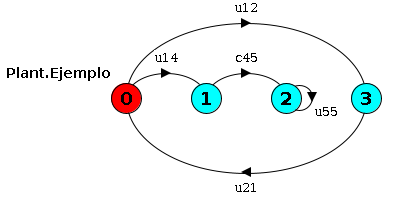
\includegraphics[scale=0.7]{figures/tests/test1.png}
 \caption{LTS del test 1}
 \label{fig:test1}
\end{figure}

\smallskip
\textbf{Test 8} Fig \ref{fig:test8} 
Es un problema de falencias al encontrar errores explicado en la sección \ref{marcarErrores}. Si no se señala el estado 3 como error, porque no se detecta que es un livelock entonces podríamos sacar la conclusión errada que es controlable. Notar que esto sería lo mismo que si tenemos una rama totalmente explorada a partir de u33.
\begin{figure}[h]
 \centering
 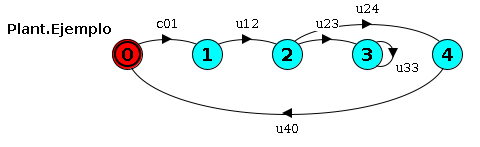
\includegraphics[scale=0.7]{figures/tests/test8.png}
 \caption{LTS del test 8}
 \label{fig:test8}
\end{figure}

\smallskip
\textbf{Test 12} Fig \ref{fig:test12}
Variante del test 8, en este caso existe controlador ya que se llega al livelock por una controlable (que puede ser desactivada). Notar que aunque el estado $1$ esté marcado es necesario dejarlo fuera para poder asegurar victoria, se ganaría gracias al estado $5$ que también está marcado (con llegar a uno de ellos alcanza). 
\begin{figure}[h]
 \centering
 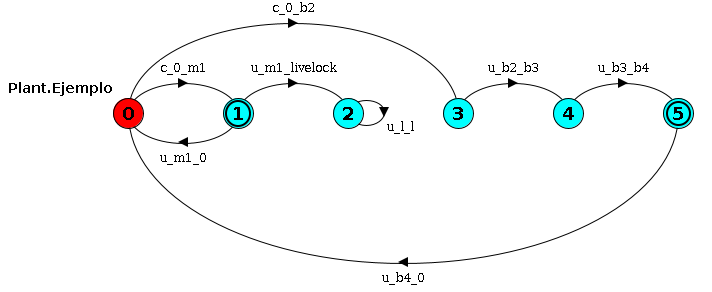
\includegraphics[scale=0.6]{figures/tests/test12.png}
 \caption{LTS del test 12}
 \label{fig:test12}
\end{figure}

\smallskip
\textbf{Test 26} Fig \ref{fig:test26} 
Otro ejemplo de por qué la propagación no puede ser local. Ambos loops no controlables son ganadores pero es necesario saber que tanto la transición $u20$ como la $u23$ se ``quedan en el conjunto de ancestros'' para poder llegar a esa conclusión.
\begin{figure}[h]
 \centering
 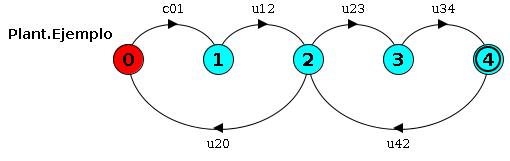
\includegraphics[scale=0.7]{figures/tests/test26.png}
 \caption{LTS del test 26}
 \label{fig:test26}
\end{figure}

\smallskip
\textbf{Test 30} Fig \ref{fig:test30} 
Caso parecido al test 26 pero ahora el estado en duda no es tan directo como antes. Esta vez $2$ y $3$ son agregados a $\Goals$ y recién podemos tener problemas al propagar a $0$. Necesitamos ver que $1$ y $0$ son parte del mismo ``conjunto controlablemente cerrado'' para notar que el autómata es controlable. %TODO ok con eso de conjunto controlablemente cerrado? o lo queremos llamar de otra manera?
\begin{figure}[h]
 \centering
 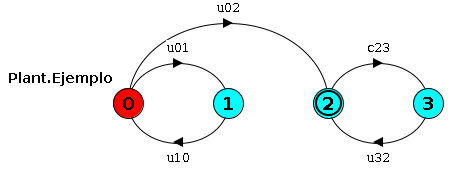
\includegraphics[scale=0.7]{figures/tests/test30.png}
 \caption{LTS del test 30}
 \label{fig:test30}
\end{figure}

%TODO seguir por acá, el 35 va? falta el resto, tampoco poner demasiados, no?.
\smallskip
\textbf{Test 35} El tema es que arma un CCC y no chequea que sea válido bien, porque ya no hay loop con marcado. Entonces el build Controller se queja y da que no hay controlador. Pero si revisaba para el otro lado había un CCC válido

%TODO agregar tests que usen debuggins abs (i.e., que tengan nombres las transiciones) Ej que puede estar muy bien: TEST 41

%TODO AGREGAR LOS TESTS QUE NOS HICIERON DAR CUENTA QUE EL PROPAGATE NO PODIA SER LOCAL Y HABIA QUE MARCAR ERRORES AL TERMINAR DE EXPLORAR ALGO

%TODO agregar los tests nuevos test 47 o 48?
